\documentclass[CJK,11pt]{amsart}
\usepackage{CJK}
\usepackage{lipsum}
\usepackage{amsfonts}
\usepackage{graphicx}
\usepackage{epstopdf}
\usepackage{algorithmic}
\usepackage{hyperref}
\hypersetup{
	colorlinks=true,
	linkcolor=blue,
	filecolor=blue,      
	urlcolor=blue,
	citecolor=cyan,
}
\ifpdf
  \DeclareGraphicsExtensions{.eps,.pdf,.png,.jpg}
\else
  \DeclareGraphicsExtensions{.eps}
\fi

% Add a serial/Oxford comma by default.
\newcommand{\creflastconjunction}{, and~}

\usepackage{amsopn}
\DeclareMathOperator{\diag}{diag}

\usepackage{relsize}
\usepackage{pxfonts}
\usepackage{tikz}
\usetikzlibrary{arrows,shapes,chains,positioning}
\usetikzlibrary{decorations.markings}
\tikzstyle arrowstyle=[scale=1]
\tikzstyle directed=[postaction={decorate,decoration={markings,mark=at position .65 with {\arrow[arrowstyle]{stealth}}}}]
\tikzstyle reverse directed=[postaction={decorate,decoration={markings,mark=at position .65 with {\arrowreversed[arrowstyle]{stealth};}}}]
\newtheorem{Def}{Definition}
\newtheorem{Th}{Theorem}[section]
\newtheorem{Lm}{Lemma}[section] 
  
\theoremstyle{definition}
\begin{document}
\begin{CJK*}{UTF8}{gbsn}
\title{
The Life and Mathematics of James H. Bramble
}
\author{Students of Bramble}
\maketitle

\section{News and family}
James Henry Bramble, one of the most distinguished computational mathematicians of all times and our beloved mentor and friend, died July 20, 2021 at his home in Austin, Texas. He was 90.

Bramble was born on December 1, 1930 in Annapolis, Maryland to Edith and Clinton Bramble. He had two sisters, Mary Aller and Barbara Lawrence, both deceased. 
In 1978, Bramble married Margaret (Peggy) Hays, (she passed away March 28, 2019). 
He is survived by his four children, Margot Dermody of Pittsburgh, Pennsylvania, Tamara Lamenzo of Needham, Massachusetts, Mitzi Bramble of Harwich, Massachusetts, and James Bramble of Austin, his step-son, Alan Hays of Ithaca, and eight grand-children. He also is survived by his first wife, Mary Eppie Boze. 

{\color{red} He earned his bachelor degree from Brown University in
  1953, a Master's degree and Ph.D. degree from the University of
  Maryland in 1955 and 1958 respectively.  After working for General
  Electric and the Naval Ordnance Laboratory, he became a professor at
  the University of Maryland.  In 1968, he was recruited to Cornell.}

After retiring from Cornell in 1994 and then retiring from Texas A\&M
in 2007, Bramble and his wife, Peggy, remained in Austin, but returned
to their lakeside cottage in Ithaca every summer.  They enjoyed
entertaining friends and family, playing golf and tennis, and boating.

He will be remembered fondly by family, friends, and colleagues worldwide.

\subsection{Cornell days}
In his 26 years at Cornell, as professor of Mathematics in the College of Arts and Sciences,  Bramble helped move his department to the forefront of applied mathematics and became a leading figure in his field, bridging rigorous theory and practical numerical computation.  “Cornell hired Professor Bramble to help establish a world-class group in numerical analysis,” said Tara Holm, professor of mathematics and department chair. “That group began with his adviser, Larry Payne, and later included professors Lars Wahlbin and Al Schatz. Bramble was one of the top three in his field in the country and of worldwide renown. He put applied mathematics at Cornell on the world map, as it were. Bramble's work remains central in applied mathematics and continues to be highly cited today.”

Bramble also made a significant impact with Cornell's Center for Applied Mathematics. He served as its director from 1975-81, helping to secure university funding for graduate students.  In addition, Bramble served as associate chair and director of undergraduate studies in the Department of Mathematics for three years, and as graduate faculty representative in mathematics for three years, Holm said.

\subsection{Texas A\&M}
In 1994, Bramble retired from Cornell as professor emeritus. He continued his career at Texas A\&M University, where he retired in 2007 as Distinguished Professor Emeritus. 

He was an editor of the journal {\it Mathematics of Computation} for 25 years, and chief editor from 1975-83. He received an honorary doctorate from Chalmers University of Technology in Sweden in 1985 in recognition of his important contributions to mathematics.

In 1970, along with Ivo Bab{\u u}ska and Bruce Kellog, Bramble
co-founded the Finite Element Circus
(https://sites.google.com/view/fecircus), a regular meeting devoted to
the theory and applications of the finite element method and related
areas of numerical analysis and partial differential equations.  In
the early years, meetings were held as often as four times a year, but
soon a format was established of a one-and-one-half day meeting held
every spring and fall at varying locations.  The Finite Element Circus
has played a critical role in making the finite element method one
of the major numerical methods for solving partial differential
equations, and in training generations of researchers in the finite
element method.

\subsection{Ph.D. students of Bramble}
Bramble taught numerous undergraduate and graduate students, mentored
22 Ph.D. students, and had {\color{red} research collaborators}
throughout the world. Here is a list:
% % Selina help with this file
\begin{enumerate}
\item \href{https://www.linkedin.com/in/maxine-rockoff-394b114/}{Maxine Rockoff}(University of Pennsylvania, 1964), currently an adjunct associate research scientist at Columbia University.
\item \href{http://euclid.colorado.edu/~gustafs/}{Karl Gustafson}(University of Pennsylvania, 1965), currently a professor of mathematics at University of Colorado Boulder.
\item \href{https://cs.uwaterloo.ca/~rbsimpso/RBScv.pdf}{Richard Bruce Simpson}(University of Maryland, 1966), used to be a professor of computer science at uniersity of Waterloo, passed away in 2020.
\item \href{https://ep.jhu.edu/faculty/james-kuttler/}{James Kuttler}(University of Maryland, 1967), currently an instructor in JHU Whiting School of Engineering.
\item \href{https://en.wikipedia.org/wiki/Stephen_Hilbert}{Stephan Hilbert}(University of Maryland, 1969), used to be a professor of mathematics at Ithaca College.
\item \href{https://sites.math.rutgers.edu/~falk/}{Richard Falk}(Cornell University, 1971), currently a professor of mathematics at Rutgers.
\item Thomas King(Cornell University, 1971).
\item \href{https://www.legacy.com/us/obituaries/knoxnews/name/steven-serbin-obituary?pid=120620923}{Steven Serbin}(Cornell University, 1971), used to be a professor of mathematics at University of Tennessee, passed away in 2008.
\item \href{http://www.math.buffalo.edu/mad/PEEPS/baker_gartha.html}{Garth Baker}(Cornell University, 1973), used to be a lecturer of mathematics at Bermuda College.
\item \href{https://services.math.duke.edu/~johnt/}{John Trangenstein}(Cornell University, 1975), currently a professor of mathematics at Duke University.
\item \href{https://www.math.tamu.edu/~joe.pasciak/}{Joseph E. Pasciak}(Cornell University, 1977), currently a professor of mathematics at Texas A\&M University.
\item \href{https://www.mn.uio.no/math/english/people/aca/rwinther/}{Ragnar Winther}(Cornell University, 1977), currently a professor of mathematics at University of OSLO.
\item Peter Sammon(Cornell University, 1978).
\item \href{https://www.uah.edu/science/departments/math/faculty-staff/mark-pekker}{Mark J. Pekker}(Cornell University, 1982), currently a professor of mathematics at The University of Alabama in Huntsville.
\item \href{https://www.personal.psu.edu/jxx1/}{Jinchao Xu}(Cornell University, 1989), currently a professor of mathematics at Pennsylvania State University. 
\item Ping Lee(Cornell University, 1990).
\item Mark Hanisch(Cornell University, 1991).
\item \href{https://www.bgsu.edu/arts-and-sciences/mathematics-and-statistics/faculty-and-staff/tong-sun.html}{Tong Sun}(Texas A\&M, 1997), currently a professor of mathematics at Bowling Green State University.
\item \href{http://web.pdx.edu/~gjay/}{Jay Gopalakrishnan}(Texas A\&M, 1999), currently a professor of mathematics at Portland State University.
\item \href{http://www.math.udel.edu/~bacuta/}{Constantin Bacuta}(Texas A\&M, 2000), currently a professor of mathematics at University of Delaware.
\item \href{https://people.llnl.gov/kolev1}{Tzanio Kolev}(Texas A\&M, 2004), currently a computational mathematician at Lawrence Livermore National Laboratory.
\item \href{https://scholar.google.com/citations?user=EeWTb_wAAAAJ&hl=en}{Dimitar Trenev} (Texas A\&M, 2009), currently working at ExxonMobil Corporate Strategic Research.
\end{enumerate}

% Selina help with this file
\begin{enumerate}
\item \href{https://www.linkedin.com/in/maxine-rockoff-394b114/}{Maxine Rockoff}(University of Pennsylvania, 1964), currently an adjunct associate research scientist at Columbia University.
\item \href{http://euclid.colorado.edu/~gustafs/}{Karl Gustafson}(University of Pennsylvania, 1965), currently a professor of mathematics at University of Colorado Boulder.
\item \href{https://cs.uwaterloo.ca/~rbsimpso/RBScv.pdf}{Richard Bruce Simpson}(University of Maryland, 1966), used to be a professor of computer science at uniersity of Waterloo, passed away in 2020.
\item \href{https://ep.jhu.edu/faculty/james-kuttler/}{James Kuttler}(University of Maryland, 1967), currently an instructor in JHU Whiting School of Engineering.
\item \href{https://en.wikipedia.org/wiki/Stephen_Hilbert}{Stephan Hilbert}(University of Maryland, 1969), used to be a professor of mathematics at Ithaca College.
\item \href{https://sites.math.rutgers.edu/~falk/}{Richard Falk}(Cornell University, 1971), currently a professor of mathematics at Rutgers.
\item Thomas King(Cornell University, 1971).
\item \href{https://www.legacy.com/us/obituaries/knoxnews/name/steven-serbin-obituary?pid=120620923}{Steven Serbin}(Cornell University, 1971), used to be a professor of mathematics at University of Tennessee, passed away in 2008.
\item \href{http://www.math.buffalo.edu/mad/PEEPS/baker_gartha.html}{Garth Baker}(Cornell University, 1973), used to be a lecturer of mathematics at Bermuda College.
\item \href{https://services.math.duke.edu/~johnt/}{John Trangenstein}(Cornell University, 1975), currently a professor of mathematics at Duke University.
\item \href{https://www.math.tamu.edu/~joe.pasciak/}{Joseph E. Pasciak}(Cornell University, 1977), currently a professor of mathematics at Texas A\&M University.
\item \href{https://www.mn.uio.no/math/english/people/aca/rwinther/}{Ragnar Winther}(Cornell University, 1977), currently a professor of mathematics at University of OSLO.
\item Peter Sammon(Cornell University, 1978).
\item \href{https://www.uah.edu/science/departments/math/faculty-staff/mark-pekker}{Mark J. Pekker}(Cornell University, 1982), currently a professor of mathematics at The University of Alabama in Huntsville.
\item \href{https://www.personal.psu.edu/jxx1/}{Jinchao Xu}(Cornell University, 1989), currently a professor of mathematics at Pennsylvania State University. 
\item Ping Lee(Cornell University, 1990).
\item Mark Hanisch(Cornell University, 1991).
\item \href{https://www.bgsu.edu/arts-and-sciences/mathematics-and-statistics/faculty-and-staff/tong-sun.html}{Tong Sun}(Texas A\&M, 1997), currently a professor of mathematics at Bowling Green State University.
\item \href{http://web.pdx.edu/~gjay/}{Jay Gopalakrishnan}(Texas A\&M, 1999), currently a professor of mathematics at Portland State University.
\item \href{http://www.math.udel.edu/~bacuta/}{Constantin Bacuta}(Texas A\&M, 2000), currently a professor of mathematics at University of Delaware.
\item \href{https://people.llnl.gov/kolev1}{Tzanio Kolev}(Texas A\&M, 2004), currently a computational mathematician at Lawrence Livermore National Laboratory.
\item \href{https://scholar.google.com/citations?user=EeWTb_wAAAAJ&hl=en}{Dimitar Trenev} (Texas A\&M, 2009), currently working at ExxonMobil Corporate Strategic Research.
\end{enumerate}


\section{Scientific contributions}


Bramble began his research career developing analytical methods for
partial differential equations -- that is, equations that relate
functions and their derivatives.  In most of his career, he worked on
numerical solutions of partial differential equations and multigrid
method. His early work involved the mathematical analysis of finite
difference methods for elliptic problems. His later work was more
focused on the numerical analysis of finite element methods.  He also
worked on questions concerning rapid solution of large-scale systems
that result from such approximations. A typical question is: Among all
the theoretically good approximations to a general class of problems,
are there some that can be solved efficiently by taking advantage of
modern computer architectures such as parallelism? Answers to
questions like this one can bring many problems into the realm of
practical feasibility. He designed approximations to solutions to
problems in partial differential equations that adequately describe
the problem and that can be efficiently solved using modern computing
power. In particular, he was interested in Maxwell's Equations and acoustics,
including scattering problems.

A partial list of his major research interests include:
\begin{enumerate}
\item Finite difference methods
\item Finite element method
\begin{enumerate}
\item Bramble-Hilbert Lemma and error analysis
\item Super-convergence
\end{enumerate}
\item Domain decomposition methods 
\begin{enumerate}
\item Non-overlapping domain decomposition method
\item Overlapping domain decomposition method
  \end{enumerate}
\item Multigrid methods 
\item PML methods {\color{red} PML methods}
\end{enumerate}
\subsection{Finite difference method}
Dr. Bramble worked on the mathematical analysis of numerical methods
for partial differential equations. In the 1960s, he helped pioneer
the mathematical analysis of finite difference methods for elliptical
problems.

In a sequence of papers from 1962 to 1966,
\cite{bramble1962formulation, bramble1963fourth, bramble1964finite,
  bramble1965finite,bramble1965approximation,bramble1966second,bramble1966error},
Bramble and collaborators had systematical studies on error analysis
for finite difference methods for elliptic boundary value problems of
both 2nd and 4th order with various different (Dirichlet, Neumann and
mixed) boundary conditions.  For example, by using the discrete maximum
principle, he proved that the finite difference schemes for domains
with curved boundaries still have $\mathcal O(h^2)$ accuracy, despite the
fact the truncation error is only of order $\mathcal (h)$ near the
boundary.  As another example, in paper \cite{bramble1964finite}, he
provided a special example in which the matrix is neither
diagonally dominant nor of non-negative type, but for which a maximum
principle still holds. This is a deep observation about the maximum
principle for finite difference methods.

% \chapter{Finite Difference Methods}

\section{On the formulation of finite difference analogues of the Dirichlet problem for Poisson's equation (1962)}
On the formulation of finite difference analogues of the Dirichlet problem for Poisson's equation \cite{bramble1962formulation}
\includepdf[pages = 2-]{Papers/FDM/bramble1962formulation.pdf}

\section{Fourth-order finite difference analogues of the Dirichlet problem for Poisson's equation in three and four dimensions (1963)}
Fourth-order finite difference analogues of the Dirichlet problem for Poisson's equation in three and four dimensions \cite{bramble1963fourth}

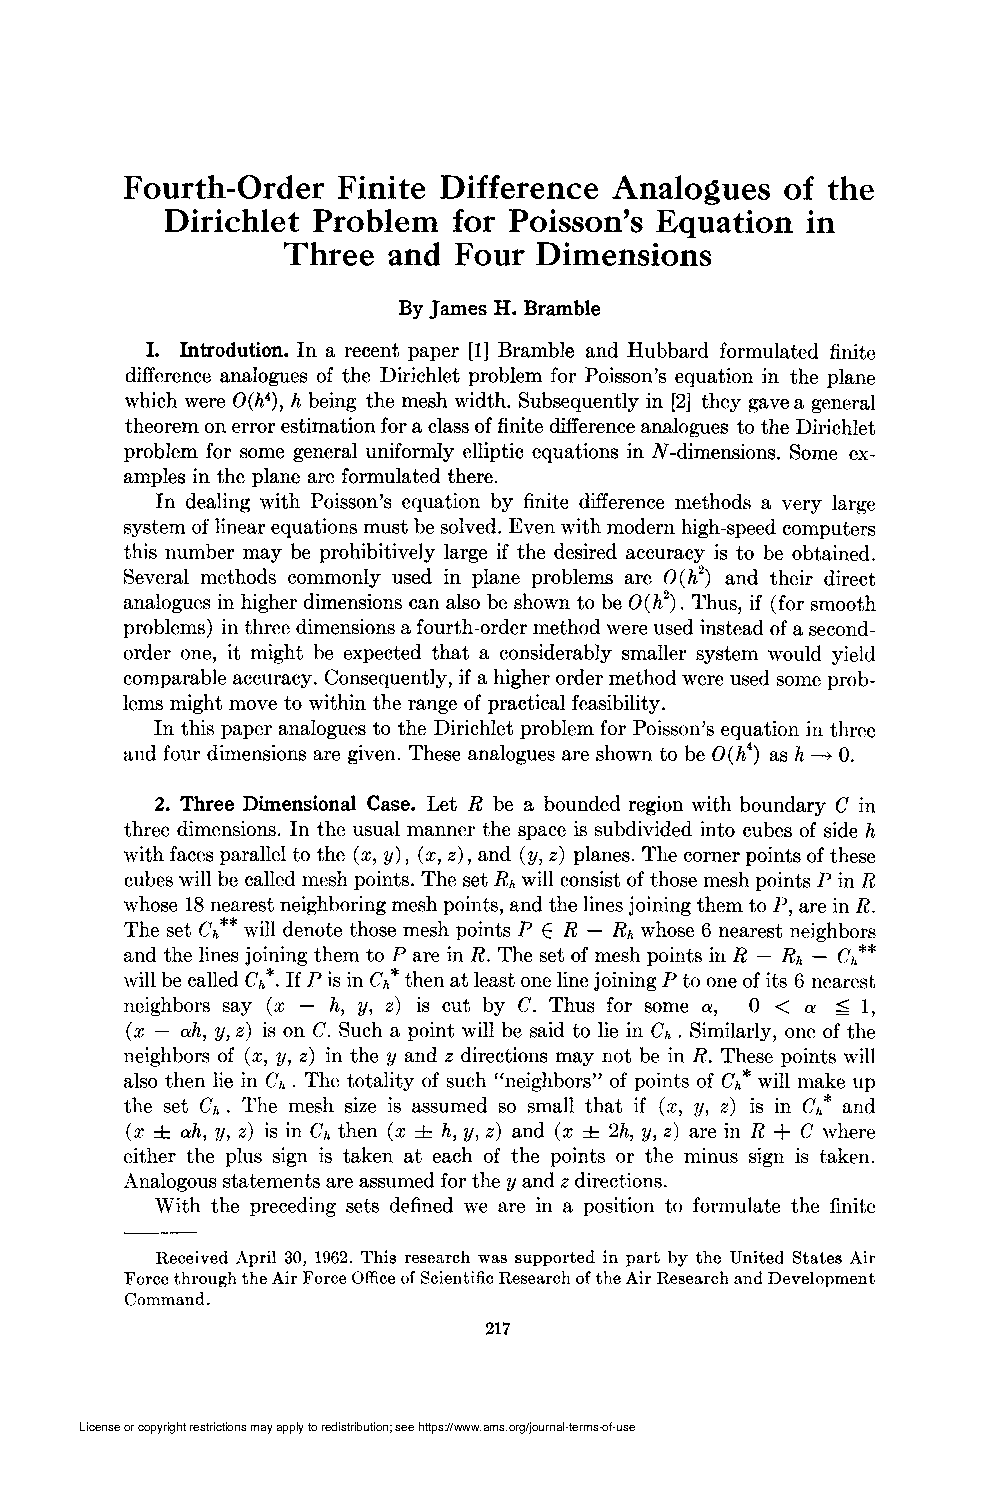
\includepdf[pages = -]{Papers/FDM/bramble1963fourth.pdf}


\section{New monotone type approximations for elliptic problems (1964)}
New monotone type approximations for elliptic problems\cite{bramble1964new}
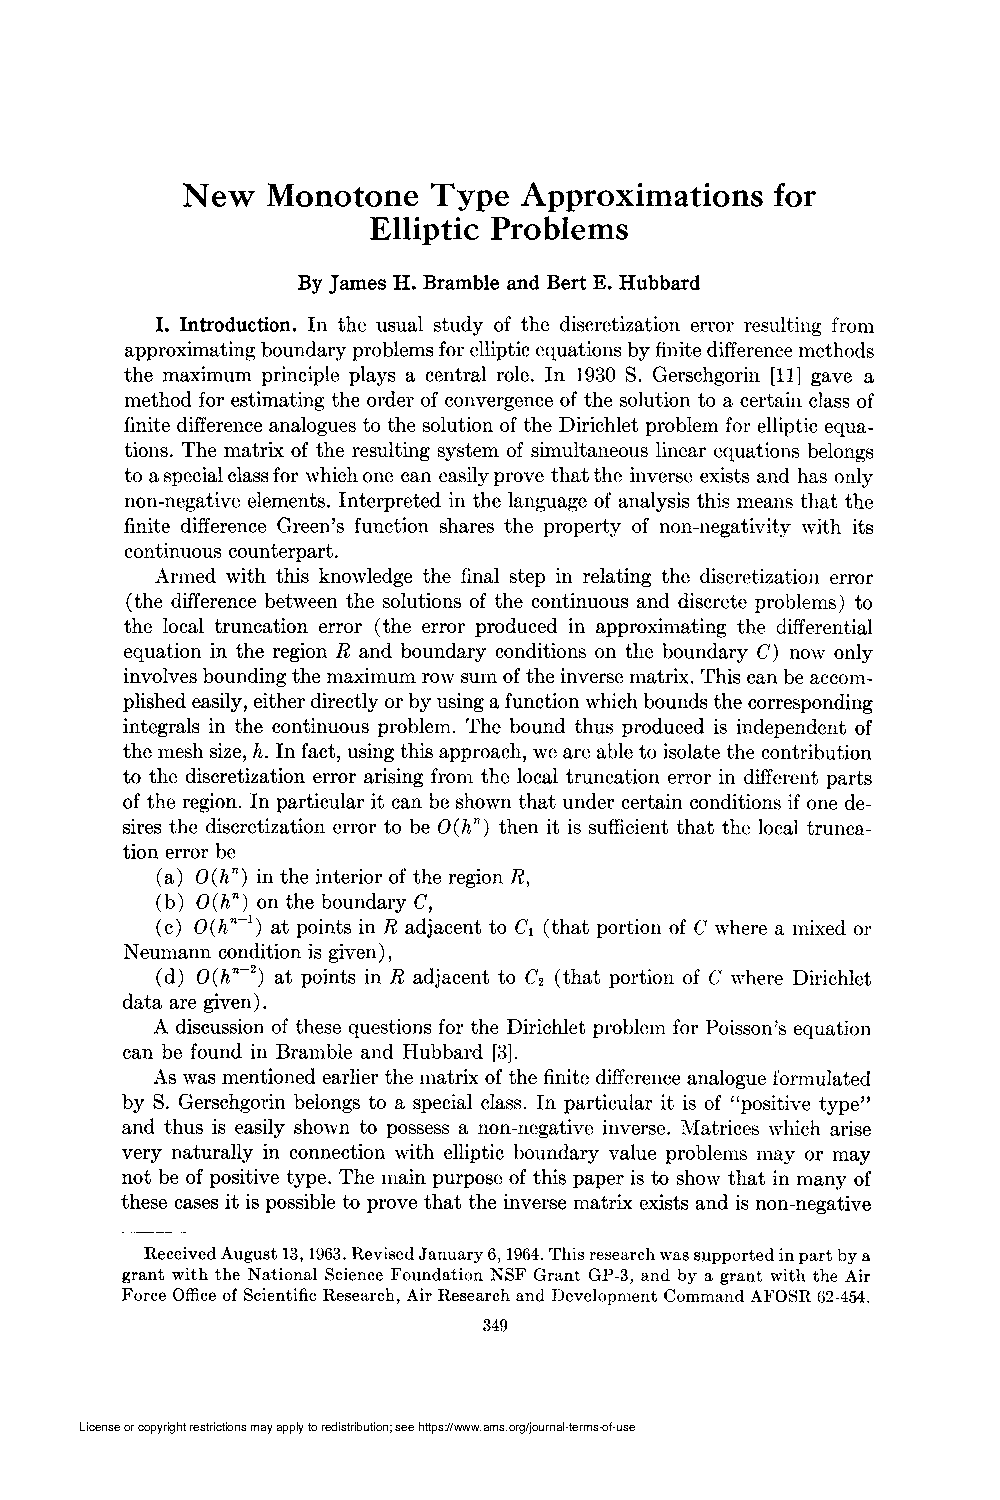
\includepdf[pages = -]{Papers/FDM/bramble1964new.pdf}

\section{On a finite difference analogue of an elliptic boundary problem which is neither diagonally dominant nor of non-negative type (1964)}

On a finite difference analogue of an elliptic boundary problem which is neither diagonally dominant nor of non-negative type \cite{bramble1964finite}

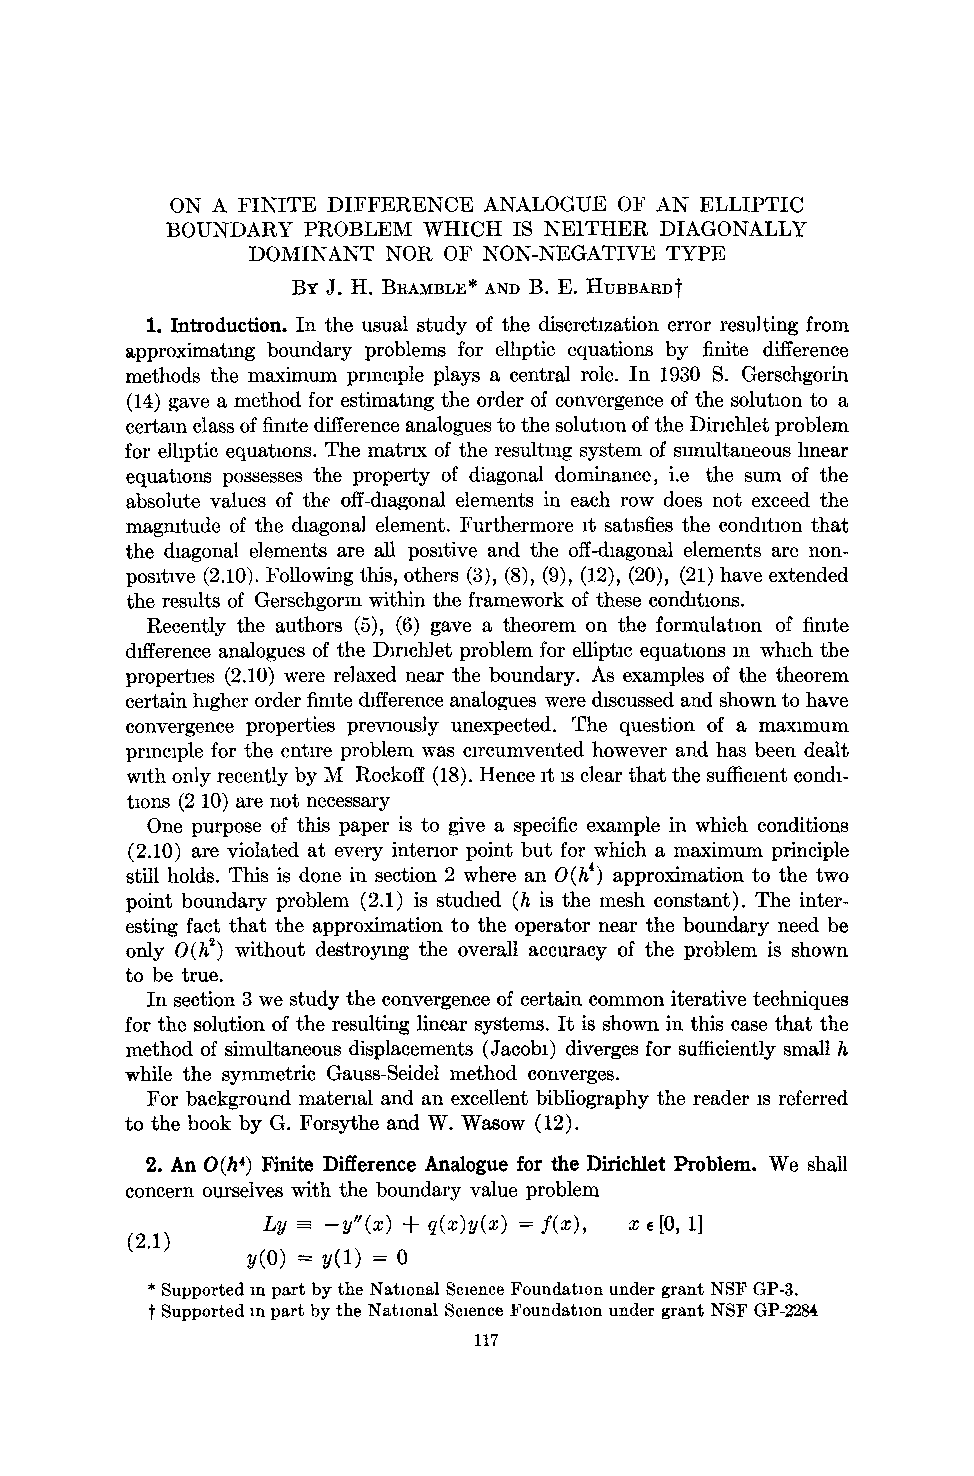
\includepdf[pages = -]{Papers/FDM/bramble1964finite.pdf}

\section{Approximation of solutions of mixed boundary value problems for Poisson's equation by finite differences (1965)}

Approximation of solutions of mixed boundary value problems for Poisson's equation by finite differences \cite{bramble1965approximation}

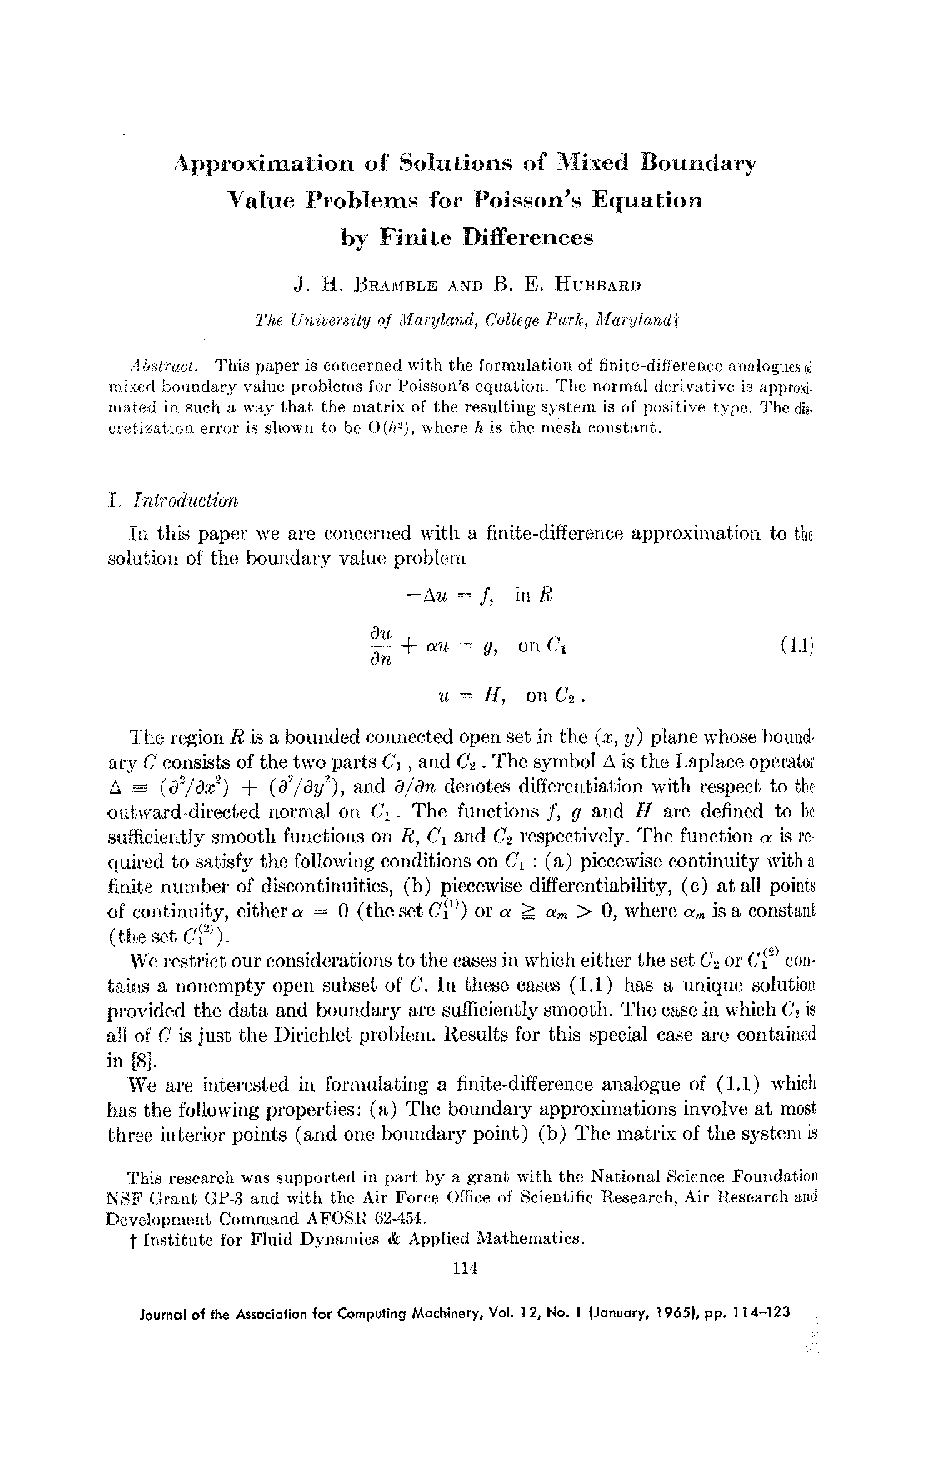
\includepdf[pages = -]{Papers/FDM/bramble1965approximation.pdf}

\section{A finite difference analog of the Neumann problem for Poisson's equation (1965)}
A finite difference analog of the Neumann problem for Poisson's equation \cite{bramble1965finite}

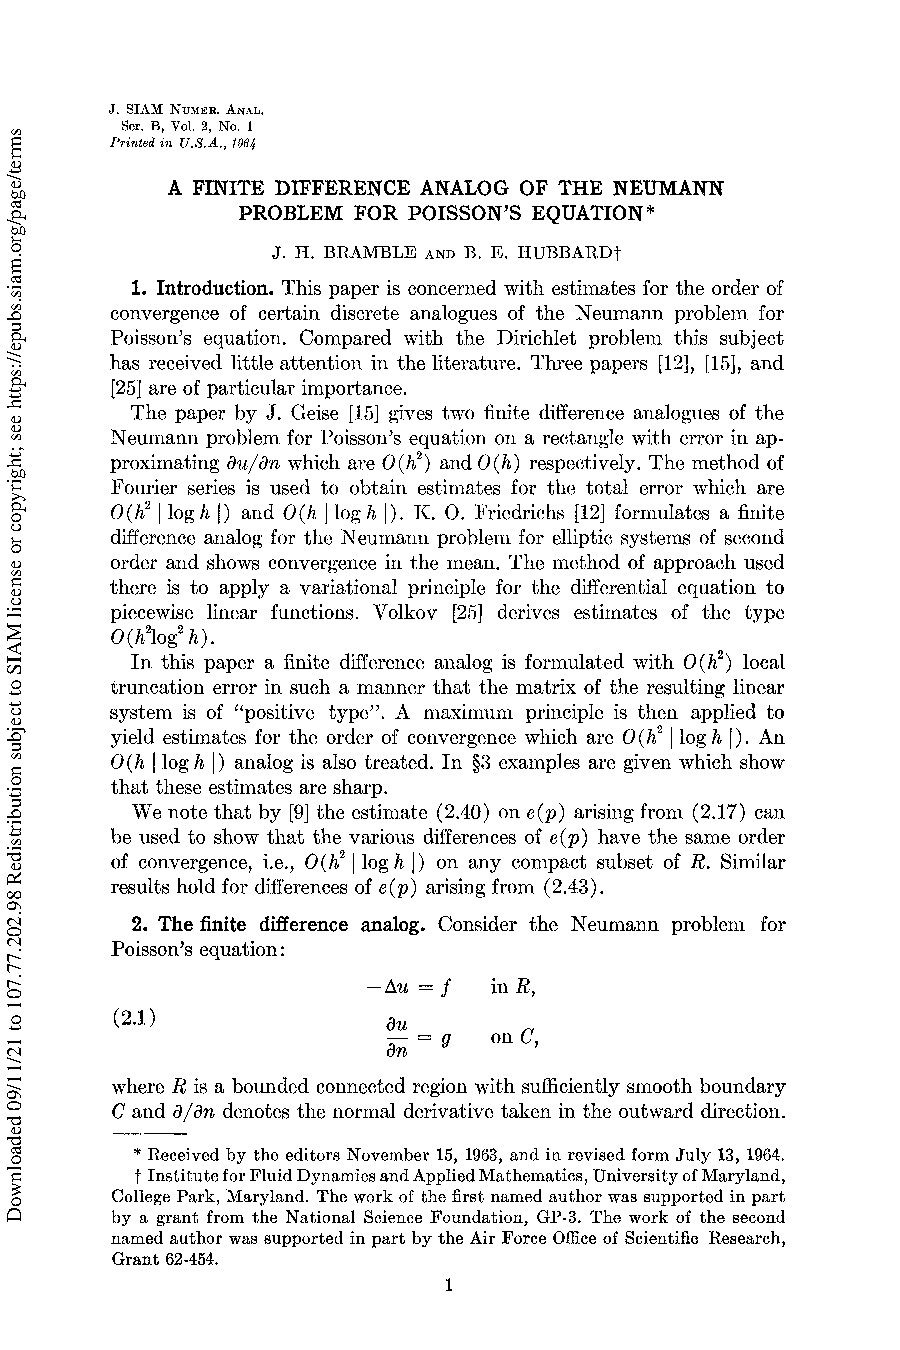
\includepdf[pages = -]{Papers/FDM/bramble1965finite.pdf}

\section{A second order finite difference analog of the first biharmonic boundary value problem (1966)}
A second order finite difference analog of the first biharmonic boundary value problem \cite{bramble1966second}
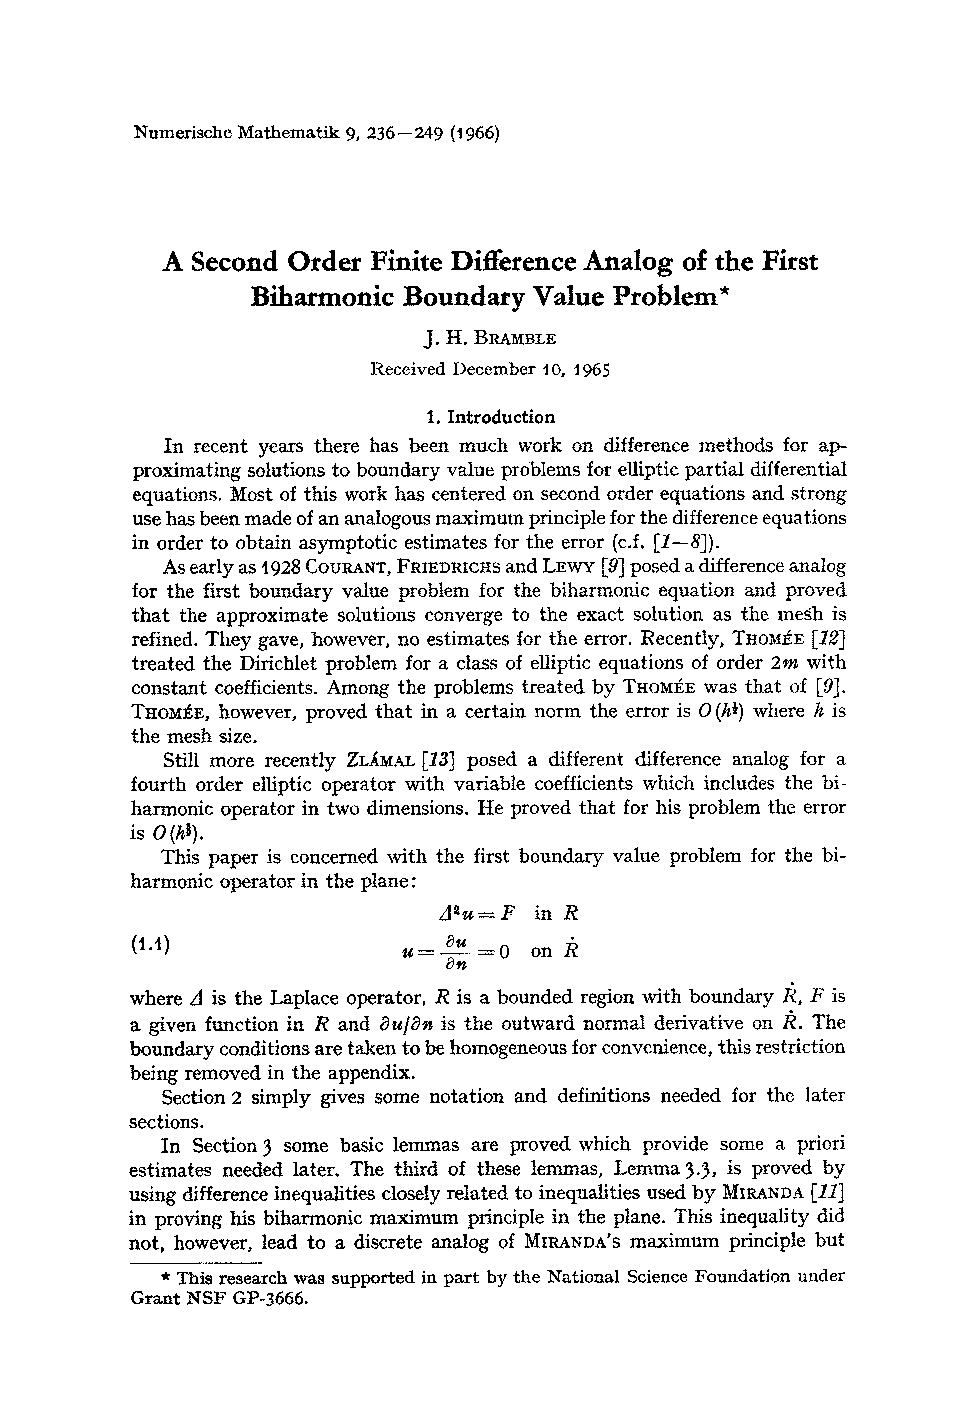
\includepdf[pages = -]{Papers/FDM/bramble1966second.pdf}

\section{Error estimates for difference methods in forced vibration problems (1966)}
Error estimates for difference methods in forced vibration problems \cite{bramble1966error}
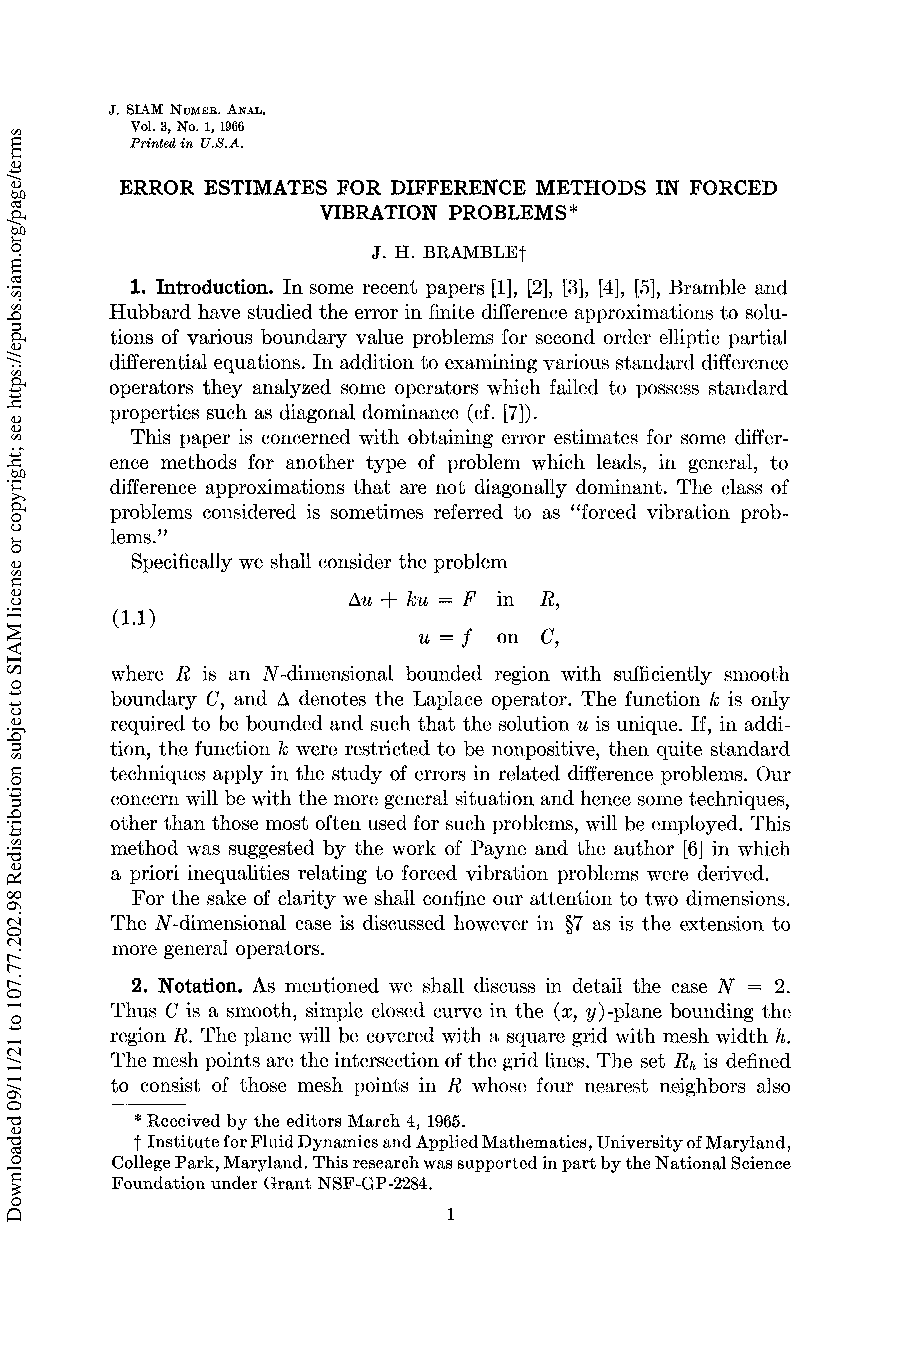
\includepdf[pages = -]{Papers/FDM/bramble1966error.pdf}

\section{On the convergence of difference approximations to weak solutions of Dirichlet's problem (1969)}
On the convergence of difference approximations to weak solutions of Dirichlet's problem \cite{bramble1969convergence}
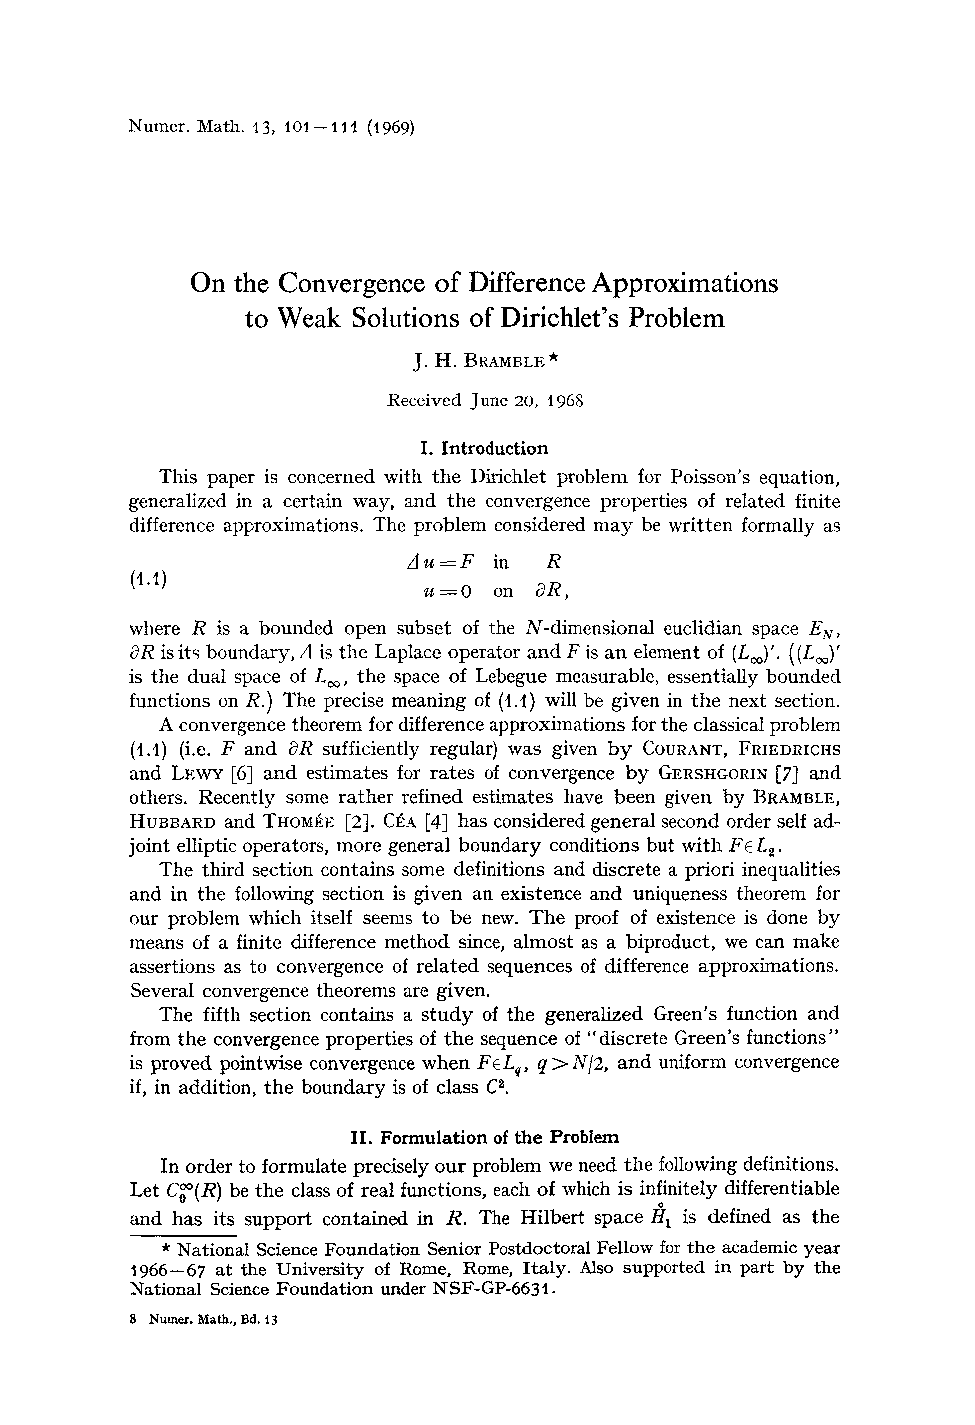
\includepdf[pages = -]{Papers/FDM/bramble1969convergence.pdf}

%\subsection{Finite difference method}
Finite difference method was extended and analyzed by Dr. Bramble for Dirichlet problem of Poisson's equation on a domain with curve boundary \cite{bramble1962formulation}, and then  for Neumann problem of Poisson's 
equation on a domain with curve boundary \cite{bramble1965finite}, and approximation of solutions of mixed boundary value problems for Poisson's equation by finite difference method was also considered by Dr. Bramble in \cite{bramble1965approximation}.   Even further, Dr. Bramble considered and analyzed higher order finite difference method for bounded  domain in higher dimension, such as fourth-order finite difference analogues of the Dirichlet problem for Poisson's equation in three and four dimensions were consider in \cite{bramble1963fourth}. 

A second order finite difference analog of the first biharmonic boundary value problem was also done by Dr. Bramble in \cite{bramble1966second}. 
Error estimates for finite difference methods for indefinite problem such as in forced vibration problems was also given by Dr. Bramble in \cite{bramble1966error}. In paper \cite{bramble1964finite}, Dr. Bramble showed  a special example in which case the matrix is neither diagonally dominant nor of non-negative type, but for which a maximum principle still holds. This is a deep observation of the maximum principle of finite difference methods.  

\subsection{Finite element method}
In the ensuing decades, one of the major focuses of Bramble's research
was the development and analysis of the finite element method, and
especially its theoretical foundations, applied to the approximation
of solutions of elliptic and parabolic partial differential equations.

\subsubsection{Bramble-Hilbert lemma}
One of his most famous results, the Bramble-Hilbert Lemma, a
theoretical tool for proving error estimates for the finite element
method, was a collaborative effort with his Ph.D. student, Stephen
Hilbert \cite{bramble1970estimation}.

The Bramble-Hilbert Lemma states that for any bounded functional
$F:W^{m,p}(\Omega)\mapsto\mathbb R$ that annihilates polynomials of
degrees $m-1$, then $F(v)\le C|v|_{m,p,\Omega}$ for any $v\in
W^{m,p}(\Omega)$.  What is equally important, as demonstrated in the
original paper \cite{bramble1970estimation}, is how this Lemma is
used together with a scaling argument to derive error estimates in Sobolev norms for
approximation of smooth functions by finite elements.  This
gives a very general and very elegant way to derive error estimates
for piecewise polynomial approximation, for numerical quadrature and for
many other applications.  It is a basic tool for finite element error
analysis and used by every researcher in this field.

\subsubsection{The eigenvalue problems} Together with John Osborn, Jim developed in \cite{bramble1973rate}  error estimates for the approximating the  eigenvalues of nonself-adjoint operators.
 Various methods for defining the approximate eigenvalues are treated, including methods in which the functions in the subspaces of trial functions are not required to satisfy any boundary conditions. The estimates are optimal in the sense that they give the best estimate that could be expected on the basis of the approximability properties of the underlying subspaces. The work extends on previous results on obtaining lower bounds for the inverse Poincare  constant and estimating first nonzero Steklov eigenvalue for second order elliptic PDEs, \cite{bramble1962bounds}. 

\subsubsection{Time-steping methods}  For second order hyperbolic equations, a new class of single step fully discrete schemes is developed. The schemes  are high order accurate in time,  \cite{baker1979semidiscrete}.  Together with Baker and Thom\'{e}e in \cite{baker1977single} convergence estimates for semidiscrete  approximations for Parabolic Equations
are investigated. The results include $L_2 $  and maximum norm estimates,  and superconvergence estimates.  Several of the estimates are derived  under weak assumptions on the initial data.



\subsubsection{Post-processing and super-convergence} In
\cite{bramble1977higher} together with Schatz, {\it superconvergence}
results for a class of Ritz-Galerkin methods for approximating
elliptic boundary problems are developed.  Convolution operators with
locally supported functions are designed that are easy to compute from
the Ritz-Galerkin approximation and lead to higher order of
approximation of the solution in both $L^2$ and $L^\infty$ norms for
translation invariant grids.  This convolutional operator does not
depend on the specific elliptic operator and is easily constructed.
This technique of using convolution operator for translation invariant
grids is reminiscent of the convolutional neural network~\cite{lecun1998gradient} for
classification of image, which was also motivated by the fact that the
main feature of an image is translational invariant.



\subsection{Domain decomposition methods}
Domain decomposition methods can be, roughly speaking, divided into
two different classes: (1) non-overlapping domain decomposition
methods, and (2) overlapping domain decomposition methods.  In both
classes of methods, Bramble has made fundamental contributions.

\subsubsection{Non-overlapping domain decomposition methods}
In the sequence of 4 papers \cite{bramble1986construction, bramble1987construction, bramble1988construction, bramble1989construction}, Bramble, Pasciak and Schatz gave a systematic development of basic non-overlapping domain decomposition methods, including an estimate of 
the condition number of the resulting preconditioned systems. 

\subsubsection{Overlapping domain decomposition methods}
Overlapping domain decomposition methods can be traced back to Schwarz
\cite{} for the two subdomain case.  In his original paper, Schwarz
also provided a convergence analysis using the maximum principle (???).
In ???, Lions used a variational approach to give a convergence
analysis in the context of Sobolev space $H^1$ for the two-subdomain
case.


In \cite{bramble1991convergence-b}, the first optimal convergence
analysis is given for the overlapping domain decomposition methods
with coarse space.

 {\color{red} research collaborators}

\subsection{Multigrid and multilevel methods}

\subsubsection{Multigrid methods}  Multigrid methods are among the most efficient iterative methods for
the solution of linear systems which arise in many large scale
scientific calculations. Every researcher working with the numerical
solution of partial differential equations should at least be familiar
with these powerful techniques. Multigrid methods can be traced back to
the early seventies.  An early and major advocate of multigrid
method was A. Brandt.   A uniform convergence analysis for
a multigrid method for 2nd order elliptic boundary value problems was
provided by Bank and Dupont \cite{}.  A mathematical foundation of the multigrid method
was set up by Hackbusch and his collaborators \cite{}. An invaluable contribution
to this field is Bramble's book {\it Multigrid Methods} \cite{bramble2019multigrid}, which 
presents results concerning the rates of convergence of multigrid iterations.

\subsubsection{Multilevel representation of norms and applications}
Based on the general multilevel foundation used for multigrid methods
and using real method of interpolation theory, together with Pasciak,
Xu, and Bacuta, in a series of five papers,
\cite{bacuta2002shift, bacuta2003using, bacuta2003regularity-c, bacuta2003regularity-a, bacuta2003regularity-b}, a
new approach was developed for obtaining sharp stability estimates
(using fractional norms) for certain elliptic boundary value
problems. In \cite{bacuta2002shift, bacuta2003using}
new interpolation results that generalizes Kellogg's subspace
interpolation theory are developed for proving regularity estimates
for the Laplace and Biharmonic operators. Regularity for the Poisson
equation on non-convex polygonal domains at the the critical case are
investigated in \cite{bacuta2003regularity-c, bacuta2003regularity-a}.
For the plane elasticity problem on a convex polygonal domains
regularity is proved with constants independent of the Lam?e
coefficients, \cite{bacuta2003regularity-b}.

 
\bibliographystyle{plain}
\bibliography{bramble.bib}

\end{CJK*}
\end{document}



